\documentclass[twocolumn,10pt]{article}

\usepackage[utf8]{inputenc}
\usepackage{lmodern}
\usepackage[margin=0.7in, columnsep=0.25in]{geometry}
\usepackage{amsmath,amssymb,amsfonts,amsthm}
\usepackage{booktabs}
\usepackage{xcolor}
\usepackage{titlesec}
\usepackage{tcolorbox}
\usepackage{tikz}
\usetikzlibrary{shapes.geometric, arrows.meta, positioning}
\usepackage{hyperref}
\usepackage{caption}
\usepackage{mathtools}
\usepackage{graphicx}

% Color Palette - Formal academic with a modern, engaging twist
\definecolor{primary}{HTML}{1E293B}     % Deep Slate Navy
\definecolor{accent}{HTML}{160F99}      % Vibrant Teal Accent
\definecolor{highlight}{HTML}{A31A28}   % Crimson Highlight
\definecolor{bglight}{HTML}{F8FAFC}     % Crisp Off-White / Light Slate
\definecolor{codebg}{HTML}{F1F5F9}      % Light Code Block Background
\definecolor{bordergrey}{HTML}{CBD5E1}  % Clean Light Grey Border

% Hyperlink configuration
\hypersetup{
    colorlinks=true,
    linkcolor=accent,
    citecolor=accent,
    urlcolor=highlight
}

% Section Heading Styling (Fun but Formal)
\titleformat{\section}
  {\color{primary}\large\bfseries}
  {\thesection.}
  {0.5em}
  {}
  [\color{accent}\titlerule]

\titleformat{\subsection}
  {\color{primary}\normalfont\bfseries}
  {\thesubsection}
  {0.5em}
  {}

% Custom Callout & Accent Boxes using tcolorbox
\tcbuselibrary{skins, breakable}

% Key Insight Callout Box
\newtcolorbox{insightbox}[1][]{
  enhanced,
  colback=bglight,
  colframe=accent,
  fonttitle=\bfseries\color{white},
  coltitle=white,
  title={#1},
  arc=3pt,
  boxrule=1pt,
  left=8pt, right=8pt, top=6pt, bottom=6pt
}

% Fun Fact / Takeaway Spotlight
\newtcolorbox{funfact}[1][]{
  enhanced,
  colback=highlight!5!white,
  colframe=highlight!85!black,
  fonttitle=\bfseries\color{white},
  title={#1},
  arc=3pt,
  boxrule=0.8pt,
  left=8pt, right=8pt, top=6pt, bottom=6pt
}

% Pseudocode Box
\newtcolorbox{pseudobox}[1][]{
  enhanced,
  colback=codebg,
  colframe=primary,
  fonttitle=\bfseries\color{white},
  title={#1},
  arc=2pt,
  boxrule=0.8pt,
  left=6pt, right=6pt, top=6pt, bottom=6pt
}

% Allow large top floats to share pages with text
\renewcommand{\topfraction}{0.9}      % Up to 90% of page height can be floats
\renewcommand{\textfraction}{0.1}     % As little as 10% text on the page
\renewcommand{\floatpagefraction}{0.85}
\newcounter{myalgo}
\raggedbottom

% Title and Author Information
\title{\textbf{\Large Constraint-Aware Variable Ordering in Symbolic Optimal Planning}\\[0.5em]
\large \textcolor{accent}{Final Course Project Report -- Automatic Planning }}

\author{
  \begin{minipage}[t]{0.45\textwidth}
    \centering
    \textbf{Mozes Yaron}\\[0.4em]
    \small Faculty of Data and Decision Sciences\\
    \small Technion -- Israel Institute of Technology\\
    \small \texttt{yaron.mozes@campus.technion.ac.il}
  \end{minipage}%
  \hfill
  \begin{minipage}[t]{0.45\textwidth}
    \centering
    \textbf{Kadzelshvily Galit}\\[0.4em]
    \small Faculty of Data and Decision Sciences\\
    \small Technion -- Israel Institute of Technology\\
    \small \texttt{galit.k@campus.technion.ac.il}
  \end{minipage}
}

\date{\small August 2026 \quad $\cdot$ \quad \url{https://github.com/YaronMozes/slbd-symbolic-search-research}}

\begin{document}

\maketitle

\begin{abstract}
\noindent Symbolic BDD-based search is a prominent paradigm for cost-optimal classical planning, with its performance heavily dictated by BDD sizes and, consequently, variable ordering algorithms. State-of-the-art planners such as \textsf{SymK} rely on causal-graph proximity heuristics (e.g., \textsf{GAMER}) but ignore the structural impact of mutex and invariant constraint BDDs conjoined at every search step. We introduce constraint-aware variable ordering - incorporating mutex and invariant co-occurrence edges into the \textsf{GAMER}-family linear arrangement objective - and evaluate its impact across the complete IPC optimal-STRIPS suite within \textsf{SymK} (IPC-2023). We show that a targeted per-domain policy strictly improves stock \textsf{SymK}'s coverage on its five target domains, replicated across independent runs, and yields substantial search acceleration in domains such as \textit{woodworking}. Suite-wide, however, enabling the ordering universally results in a tightly bounded null effect. In-depth diagnostic logging explains this discrepancy: while the ordering successfully shrinks transition relations, transition relation size is largely decoupled from search cost, which is instead dominated by peak search-BDD size. Finally, we highlight key methodological pitfalls, including regression to the mean in "hard instance" subsets and cross-year IPC duplicate leakage in domain-wise cross-validation.
\end{abstract}

\section{Introduction}
Cost-optimal classical planning aims to find provably minimal-cost plan sequences in deterministic state spaces. A dominant paradigm for blind optimal planning is symbolic search, which represents sets of reachable states and transition relations compactly as Binary Decision Diagrams (BDDs) \cite{torralba2014symba}. Because symbolic search operations scale with the physical node counts of the underlying BDDs rather than the raw number of states, search efficiency is strictly governed by BDD size \cite{kissmann2014bdd}. BDD sizes, in turn, depend critically (and often exponentially) on the choice of state variable ordering \cite{kissmann2014bdd}. Modern state-of-the-art symbolic planners, including \textsf{SymK} \cite{speck2020symk, speck2023symkipc} -- which serves as the symbolic search component of \textsf{Ragnarok}, the winner of the IPC-2023 optimal track \cite{drexler2023ragnarok, taitler2024ipc} -- inherit variable ordering algorithms directly from the \textsf{GAMER} family \cite{edelkamp2008gamer}. These algorithms compute variable orders by minimizing a weighted linear arrangement objective over edges of causal-graph proximity \cite{edelkamp2008gamer}.

In addition to causal transitions, modern symbolic planners heavily rely on state-invariant constraints \cite{torralba2013constrained,torralba2017efficient}. In particular, $h^2$ mutexes and exactly-one invariant groups are compiled into constraint BDDs that are conjoined into the search frontier at every expansion step to prune reachable spurious states \cite{torralba2013constrained,torralba2017efficient}. The node sizes of these constraint BDDs depend on the same variable ordering, yet standard causal-graph ordering objectives completely ignore them \cite{torralba2013constrained}. Over a decade ago, Torralba and Alc\'azar \cite{torralba2013constrained} identified this gap and explicitly proposed incorporating mutex and invariant constraints into the variable-ordering objective as a key direction for future work. Surprisingly, to our knowledge, this suggestion has remained unverified and unevaluated in state-of-the-art planning systems \cite{torralba2013constrained}.

\begin{insightbox}[Core Research Question]
Can conjoining mutex and invariant co-occurrence edges into the \textsf{GAMER} variable ordering objective systematically compress constraint BDDs and accelerate state-of-the-art symbolic search in \textsf{SymK}?
\end{insightbox}

In this work, we implement and systematically evaluate constraint-aware variable ordering inside \textsf{SymK} on the complete IPC optimal-STRIPS benchmark suite (66 domains, 1,847 instances). During our implementation, we also identified and repaired a long-standing defect in the deployed \textsf{GAMER} ordering optimizer within \textsf{SymK}, wherein edge weights were silently ignored during local search swaps.

Across extensive empirical evaluations on the complete IPC optimal-STRIPS suite, we show that a targeted, pre-registered per-domain policy strictly improves stock \textsf{SymK} by $+6$ coverage on its five target domains (exactly replicated) while accelerating domains like \textit{woodworking} by $1.55\times$. Enabled universally, however, the ordering produces a tightly bounded null effect because it compresses transition relations without shrinking peak search-BDD sizes, the true runtime bottleneck. We present our full empirical results, diagnostic mechanism analysis, ceiling bounds, and methodological findings in Section~\ref{sec:res}.


\section{Problem Formulation}

We formalize symbolic optimal classical planning under $\text{SAS}^+$ tasks, the mechanics of constraint-conjoined BDD search, and the causal variable ordering optimization framework.

\subsection{$\text{SAS}^+$ Planning and Invariants}
A classical planning task in $\text{SAS}^+$ representation is defined as a tuple $\Pi = \langle \mathcal{V}, \mathcal{A}, s_0, s_g, \text{cost} \rangle$ \cite{kissmann2014bdd}:
\begin{itemize}
    \item $\mathcal{V} = \{v_1, \dots, v_n\}$ is a finite set of state variables. Each variable $v \in \mathcal{V}$ has a finite domain $\mathcal{D}(v)$. A \emph{fact} is a pair $(v, d)$ with $d \in \mathcal{D}(v)$.
    \item A \emph{state} $s$ is a complete assignment to $\mathcal{V}$, where $s(v) \in \mathcal{D}(v)$ for all $v \in \mathcal{V}$. The state space is denoted $\mathcal{S} = \prod_{v \in \mathcal{V}} \mathcal{D}(v)$.
    \item $s_0 \in \mathcal{S}$ is the initial state, and $s_g$ is a partial state assignment representing the goal condition.
    \item $\mathcal{A}$ is a finite set of actions. Each action $a \in \mathcal{A}$ is a pair $a = \langle \text{pre}(a), \text{eff}(a) \rangle$, where $\text{pre}(a)$ and $\text{eff}(a)$ are partial assignments over $\mathcal{V}$. Action execution incurs a non-negative cost $\text{cost}(a) \in \mathbb{R}_{\ge 0}$.
\end{itemize}

\noindent An action $a$ is applicable in $s$ if $s \models \text{pre}(a)$. Applying $a$ in $s$ yields state $s' = a(s)$ where $s'(v) = \text{eff}(a)[v]$ for variables defined in $\text{eff}(a)$, and $s'(v) = s(v)$ otherwise. A \emph{cost-optimal plan} is a sequence of actions $\pi = \langle a_1, \dots, a_k \rangle$ transforming $s_0$ into a goal state $s \models s_g$ while minimizing $\sum_{i=1}^k \text{cost}(a_i)$.

In addition to causal dynamics, domain abstractions yield state invariants $I$:
\begin{enumerate}
    \item \textbf{$h^2$ Mutexes} \cite{torralba2013constrained}: Pairs of unreachable fact combinations $\mu = \{(v_i, d_i), (v_j, d_j)\}$ such that no reachable state $s \in \mathcal{S}$ satisfies $s(v_i) = d_i \land s(v_j) = d_j$.
    \item \textbf{Exactly-One Invariants} \cite{torralba2013constrained}: Subsets of facts $\mathcal{G} \subset \bigcup_{v} \{(v,d) \mid d \in \mathcal{D}(v)\}$ such that every reachable state satisfies $\sum_{f \in \mathcal{G}} \mathbb{I}(s \models f) = 1$.
\end{enumerate}

\subsection{Symbolic Search and Constraint Conjunction}
Symbolic planning algorithms represent sets of states $S \subseteq \mathcal{S}$ and transition relations $T \subseteq \mathcal{S} \times \mathcal{S}$ as Reduced Ordered Binary Decision Diagrams (BDDs) \cite{kissmann2014bdd, torralba2014symba}.

To map $\text{SAS}^+$ variables to Boolean BDD variables, each $v_i \in \mathcal{V}$ is encoded using $m_i = \lceil \log_2 |\mathcal{D}(v_i)| \rceil$ bits. Let $X = \{x_1, \dots, x_M\}$ denote the complete set of unprimed Boolean variables representing current states, where $M = \sum_{i=1}^n m_i$, and let $X' = \{x'_1, \dots, x'_M\}$ denote primed variables representing successor states.

\begin{tcolorbox}[
  enhanced,
  colback=gray!5!white,
  colframe=gray!80!black,
  fonttitle=\bfseries\color{white},
  title={Definition (Variable Ordering)},
  arc=3pt,
  boxrule=0.8pt,
  left=8pt, right=8pt, top=6pt, bottom=6pt
]
A \textbf{variable ordering} $\pi$ is a bijection $\pi: X \cup X' \to \{1, \dots, 2M\}$ specifying the linear topological sequence in which Boolean variables are evaluated along all root-to-leaf paths in the BDD.
\end{tcolorbox}

In symbolic uniform-cost search (e.g., \textsf{sym-bd} in \textsf{SymK}) \cite{speck2020symk, torralba2014symba}, forward search expands a frontier BDD $F_k(X)$ at cost level $k$. Computing successor states requires an \emph{relational product} (Image computation) conjoined with constraint BDDs \cite{torralba2013constrained}:
\begin{equation}
    F_{k+1}(X') = \exists X \left( F_k(X) \land T(X, X') \right) \land C(X')
    \label{eq:image_comp}
\end{equation}
where $T(X, X') = \bigvee_{a \in \mathcal{A}} T_a(X, X')$ represents the system transition relation, and $C(X')$ is the conjoined invariant constraint BDD compiling all $h^2$ mutexes and exactly-one groups \cite{torralba2013constrained}:
\begin{equation}
\begin{aligned}
    C(X) = &\left( \textstyle\bigwedge_{\mu \in M_{h^2}} \neg \mu(X) \right) \;\land \\
           &\left( \textstyle\bigwedge_{\mathcal{G} \in I_{\text{one}}} \text{ExactlyOne}(\mathcal{G}, X) \right)
\end{aligned}
\label{eq:constraint_bdd}
\end{equation}

\noindent BDD node sizes during the execution of Equation~\ref{eq:image_comp} are fundamentally bounded by the width of the variable ordering \cite{kissmann2014bdd}, a dependency that constraint-graph ordering heuristics such as \textsf{FORCE} exploit outside of planning \cite{aloul2003force}.

\subsection{Causal Variable Ordering Objectives (GAMER)}
State-of-the-art planners such as \textsf{SymK} \cite{speck2020symk} compute variable orderings using the \textsf{GAMER} local search framework \cite{edelkamp2008gamer, kissmann2014bdd}. \textsf{GAMER} constructs an influence graph $G_{\text{causal}} = (\mathcal{V}, E_{\text{causal}}, w_{\text{causal}})$, where edges $(v_i, v_j) \in E_{\text{causal}}$ correspond to causal dependencies (e.g., co-occurrence in action preconditions or effects).

\textsf{GAMER} determines an optimal permutation $\pi^* \in \mathcal{P}(\mathcal{V})$ by minimizing a weighted linear arrangement (WLA) energy objective \cite{edelkamp2008gamer, kissmann2014bdd}:
\begin{equation}
    \mathcal{J}_{\text{causal}}(\pi) = \sum_{\mathclap{(v_i, v_j) \in E_{\text{causal}}}} w_{\text{causal}}(v_i, v_j) \, \bigl| \pi(v_i) - \pi(v_j) \bigr|^2
    \label{eq:gamer_obj}
\end{equation}

\subsection{Problem Statement: Constraint-Aware Variable Ordering}
While Equation~\ref{eq:gamer_obj} optimizes causal variable proximity to shrink transition relations $T_a(X, X')$, it completely ignores the structural dependencies of the constraint BDD $C(X')$ in Equation~\ref{eq:constraint_bdd} \cite{torralba2013constrained}. Because $C(X')$ is conjoined into $F_k(X')$ at every search step, suboptimal variable ordering for $C(X')$ causes catastrophic intermediate BDD node expansion \cite{torralba2013constrained}.

Our goal is to formalize a generalized objective function $\mathcal{J}_{\text{combined}}(\pi)$ that incorporates constraint co-occurrence structures $E_{\text{constraint}}$ directly into the linear arrangement search:
\begin{equation}
    \mathcal{J}_{\text{combined}}(\pi) = \mathcal{J}_{\text{causal}}(\pi) + \lambda \cdot \mathcal{J}_{\text{constraint}}(\pi)
    \label{eq:combined_problem}
\end{equation}
where $\lambda \in \mathbb{R}_{\ge 0}$ parameterizes the relative weight of invariant constraints relative to causal transition dynamics. In our implementation this trade-off parameter is realized directly as the base constraint edge weight $w_{\text{co}}$ introduced in Section~\ref{sec:influence}, i.e.\ $\lambda \equiv w_{\text{co}}$ with causal edges normalized to unit weight.

\section{Methodology}

In this section, we present the architecture of \textbf{Constraint-Aware Variable Ordering} in symbolic classical search. We formalize the construction of constraint influence edges, describe group-size normalization and causal-skipping heuristics, detail our discovery and repair of a latent defect in the \textsf{GAMER} local search optimizer, and define the per-domain policy execution framework.

\subsection{Constraint-Aware Influence Graph Construction}
\label{sec:influence}
Classical \textsf{GAMER} ordering constructs an undirected influence graph $G = (\mathcal{V}, E, w)$ over $\text{SAS}^+$ variables $\mathcal{V}$ where $E$ consists solely of causal dependencies $E_{\text{causal}}$ derived from action preconditions and effects \cite{edelkamp2008gamer, kissmann2014bdd}. To optimize for the constraint BDDs conjoined during search ($C(X)$ in Equation~\ref{eq:constraint_bdd}), we expand $G$ by overlaying a set of co-occurrence edges $E_{\text{constraint}}$ derived from $h^2$ mutexes and exactly-one invariant groups \cite{torralba2013constrained}.

Let $\mathcal{M}$ denote the set of all static invariant groups. Each group $M \in \mathcal{M}$ contains a set of facts $\mathcal{F}_M = \{(v_1, d_1), \dots, (v_k, d_k)\}$. For every pair of distinct facts $(v_i, d_i), (v_j, d_j) \in \mathcal{F}_M$ with $v_i \neq v_j$, we insert an edge $(v_i, v_j)$ into $E_{\text{constraint}}$ with a base weight $w_{\text{co}} \in \mathbb{R}_{> 0}$.

Sections~\ref{sec:groupnorm} and \ref{sec:skipcausal} describe two optional refinements of this construction. Both are exposed as ablation switches and, as reported in Section~\ref{sec:policy}, \emph{neither is enabled in the pre-registered confirmed policy}; we describe them because they delimit the design space we explored.

\subsubsection{Group-Size Normalization (optional)}
\label{sec:groupnorm}
An invariant group containing $k = |\mathcal{F}_M|$ facts generates $\binom{k}{2} = \frac{k(k-1)}{2}$ variable pairs. Unnormalized, large invariant groups (e.g., domain location features where $k \ge 30$) produce $\mathcal{O}(k^2)$ edge pairs that heavily swamp the sparse causal graph $E_{\text{causal}}$. To prevent dense invariant groups from drowning out causal structure, we define a normalized edge weight $w_{\text{pair}}$:
\begin{equation}
    w_{\text{pair}}(M) = \frac{w_{\text{co}}}{\max(1, |\mathcal{F}_M| - 1)}
    \label{eq:group_norm}
\end{equation}
This caps the total accumulated influence weight contributed by any single invariant group $M$ to $\approx \frac{w_{\text{co}} \cdot k}{2}$, maintaining a balanced weight ratio between pairwise $h^2$ mutexes ($k=2$, weight $w_{\text{co}}$) and large invariant groups.

\subsubsection{Causal Edge Skipping (optional)}
\label{sec:skipcausal}
In domains with dense causal topologies (e.g., \textit{blocks-world}, where any block can interact with any other), almost every constraint pair $(v_i, v_j) \in E_{\text{constraint}}$ is already connected in $E_{\text{causal}}$. Over-constraining these pairs tightens the variable ordering excessively, restricting local search freedom and degrading search performance. We introduce an optional filtering predicate $\text{SkipCausal}(v_i, v_j)$:
\begin{equation*}
\begin{aligned}
    \text{SkipCausal}(v_i, v_j) = \mathbb{I}\bigl( &(v_i, v_j) \in E_{\text{causal}} \\
    &\lor\; (v_j, v_i) \in E_{\text{causal}} \bigr)
\end{aligned}
\end{equation*}
When enabled, constraint edges that duplicate existing causal graph adjacencies are discarded, preserving long-range constraint edges that assist sparse domains (e.g., \textit{depot}).

\subsubsection{Combined Weight Accumulation}
The total weight $w(v_i, v_j)$ between any two state variables $v_i, v_j \in \mathcal{V}$ in the combined influence graph is computed as:
\begin{equation}
\begin{aligned}
    &\ w(v_i, v_j) = w_{\text{causal}}(v_i, v_j) + \\
    &\ \sum_{M \in \mathcal{M}_{i,j}} w_{\text{pair}}(M) \cdot \bigl(1 - \text{SkipCausal}(v_i, v_j)\bigr)
\end{aligned}
\label{eq:total_weight}
\end{equation}
where $\mathcal{M}_{i,j}$ is the set of invariant groups containing co-occurring facts for variables $v_i$ and $v_j$. In the confirmed policy configuration this reduces to $w_{\text{pair}}(M) = w_{\text{co}}$ and $\text{SkipCausal} \equiv 0$.

% ---------------------------------------------------------
% PIPELINE DIAGRAM (TikZ)
% ---------------------------------------------------------
\begin{figure}[htbp]
\centering
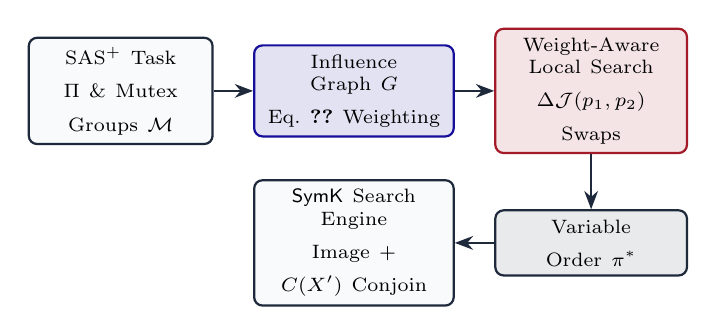
\begin{tikzpicture}[node distance=0.85cm and 0.6cm, auto, >=Stealth]
    % Nodes
    \node [draw, rectangle, rounded corners=3pt, fill=bglight, draw=primary, line width=0.8pt, text width=2.1cm, align=center] (task) {\scriptsize $\text{SAS}^+$ Task $\Pi$ \& Mutex Groups $\mathcal{M}$};

    \node [draw, rectangle, rounded corners=3pt, fill=accent!12, draw=accent, line width=0.8pt, right=0.5cm of task, text width=2.3cm, align=center] (graph) {\scriptsize Influence Graph $G$\\ Eq.~\ref{eq:total_weight} Weighting};

    \node [draw, rectangle, rounded corners=3pt, fill=highlight!12, draw=highlight, line width=0.8pt, right=0.5cm of graph, text width=2.2cm, align=center] (opt) {\scriptsize Weight-Aware Local Search\\ $\Delta \mathcal{J}(p_1, p_2)$ Swaps};

    \node [draw, rectangle, rounded corners=3pt, fill=primary!10, draw=primary, line width=0.8pt, below=0.7cm of opt, text width=2.2cm, align=center] (order) {\scriptsize Variable Order $\pi^*$};

    \node [draw, rectangle, rounded corners=3pt, fill=bglight, draw=primary, line width=0.8pt, left=0.5cm of order, text width=2.3cm, align=center] (symk) {\scriptsize \textsf{SymK} Search Engine\\ Image + $C(X')$ Conjoin};

    % Paths
    \draw[->, thick, primary] (task) -- (graph);
    \draw[->, thick, primary] (graph) -- (opt);
    \draw[->, thick, primary] (opt) -- (order);
    \draw[->, thick, primary] (order) -- (symk);
\end{tikzpicture}
\caption{System pipeline for Constraint-Aware Variable Ordering in \textsf{SymK}.}
\label{fig:pipeline_arch}
\end{figure}

\subsection{The Weight-Aware Local Search Optimizer Repair}
A critical requirement for non-uniform edge weighting (Equation~\ref{eq:total_weight}) is that the local search optimizer must faithfully evaluate edge weights during permutation steps. During our audit of the deployed \textsf{GAMER} codebase in \textsf{SymK}, we discovered a fundamental, long-standing defect in the optimizer implementation.

\subsubsection{The Deployed Defect}
In stock \textsf{GAMER} (inherited by \textsf{SymK}), the local search arrangement function evaluated edge \emph{existence} rather than edge \emph{weight}. Specifically, during the $\mathcal{O}(|\mathcal{V}|)$ incremental swap delta calculation when swapping positions of variables at index $p_1$ and $p_2$, the code checked `if (influence($v_i$, $v_j$))` as a boolean existence flag. As a result, non-unit weights $w(v_i, v_j) \neq 1.0$ were silently flattened to $1.0$. Any weighted topology blend was transformed into an unweighted graph dominated by the raw pair counts of large mutex groups.

\subsubsection{The Weight-Aware Objective Repair}
We repaired the objective function and the incremental swap delta evaluation loop. Let $\pi(p)$ denote the variable placed at topological position $p \in \{1, \dots, |\mathcal{V}|\}$. The total linear arrangement cost $\mathcal{J}(\pi)$ is defined as:
\begin{equation}
    \mathcal{J}(\pi) = \sum_{1 \le p_a < p_b \le |\mathcal{V}|} w\left(\pi(p_a), \pi(p_b)\right) \cdot (p_b - p_a)^2
    \label{eq:repaired_obj}
\end{equation}
When proposing a candidate swap between positions $p_1$ and $p_2$ (with $p_1 \neq p_2$), write $w_{k,i} \coloneqq w\bigl(\pi(k), \pi(p_i)\bigr)$ for the weight between the variable at position $k$ and the variable at swap position $p_i$. The change in objective value $\Delta \mathcal{J}(p_1, p_2)$ is then computed incrementally in $\mathcal{O}(|\mathcal{V}|)$ time:
\begin{equation}
\begin{aligned}
    \Delta \mathcal{J}(p_1, p_2) = \sum_{k \neq p_1, p_2} \Bigl[ \; &w_{k,1}\bigl( (k - p_2)^2 - (k - p_1)^2 \bigr) \\
    + \; &w_{k,2}\bigl( (k - p_1)^2 - (k - p_2)^2 \bigr) \Bigr]
\end{aligned}
\label{eq:swap_delta}
\end{equation}
If $\Delta \mathcal{J}(p_1, p_2) < 0$, the swap is accepted.

\begin{insightbox}[Backward Compatibility Guarantee]
For stock \textsf{GAMER} causal graphs, all edge weights are identically $w(v_i, v_j) = 1.0$. Consequently, Equation~\ref{eq:repaired_obj} and Equation~\ref{eq:swap_delta} yield bit-identical variable orderings to the original unweighted baseline while correctly honoring weighted topologies.
\end{insightbox}

\subsection{Algorithmic Implementation}
Algorithm~\ref{alg:constraint_ordering} details the complete variable ordering pipeline.

\begin{figure}[htbp]
\refstepcounter{myalgo}\label{alg:constraint_ordering}
\begin{pseudobox}[Algorithm \themyalgo: Constraint-Aware Variable Ordering Engine]
\small
\textbf{Input:} $\text{SAS}^+$ Task $\Pi$, Mutex Groups $\mathcal{M}$, Base Weight $w_{\text{co}}$, Iters $N_{\text{iter}}$, Restarts $R$\\
\textbf{Output:} Optimized Variable Order $\pi^*$
\begin{enumerate}\setlength{\itemsep}{0pt}\small
    \item Initialize $G = (\mathcal{V}, E, w)$ with $w(u, v) \leftarrow 0$ for all $u, v \in \mathcal{V}$
    \item \textbf{if} $\neg \text{ConstraintOnly}$ \textbf{then}
    \item \quad \textbf{for each} causal edge $(u, v) \in E_{\text{causal}}(\Pi)$ \textbf{do} $w(u, v) \leftarrow 1.0$
    \item \textbf{end if}
    \item \textbf{for each} mutex group $M \in \mathcal{M}$ \textbf{do}
    \item \quad $w_{\text{pair}} \leftarrow \text{Normalize}(w_{\text{co}}, |M|)$ via Eq.~\ref{eq:group_norm} \hfill \textit{[opt.]}
    \item \quad \textbf{for each} pair $(v_i, d_i), (v_j, d_j) \in \text{Facts}(M)$ with $v_i \neq v_j$ \textbf{do}
    \item \quad \quad \textbf{if} $\neg \text{SkipCausal}(v_i, v_j)$ \textbf{then} \hfill \textit{[opt.]}
    \item \quad \quad \quad $w(v_i, v_j) \leftarrow w(v_i, v_j) + w_{\text{pair}}$
    \item \quad \quad \textbf{end if}
    \item \quad \textbf{end for}
    \item \textbf{end for}
    \item $\pi^* \leftarrow \text{IdentityOrder}(\mathcal{V})$; \quad $\mathcal{J}^* \leftarrow \mathcal{J}(\pi^*)$ via Eq.~\ref{eq:repaired_obj}
    \item \textbf{for} $r = 0 \dots R$ \textbf{do}
    \item \quad $\pi \leftarrow (r == 0) \; ? \; \pi^* : \text{RandomPermutation}(\mathcal{V})$
    \item \quad \textbf{for} $i = 1 \dots N_{\text{iter}}$ \textbf{do}
    \item \quad \quad Sample distinct positions $p_1, p_2 \sim \text{Uniform}(1, |\mathcal{V}|)$
    \item \quad \quad Compute $\Delta \mathcal{J}(p_1, p_2)$ via Eq.~\ref{eq:swap_delta}
    \item \quad \quad \textbf{if} $\Delta \mathcal{J}(p_1, p_2) < 0$ \textbf{then} $\text{Swap}(\pi[p_1], \pi[p_2])$
    \item \quad \textbf{end for}
    \item \quad \textbf{if} $\mathcal{J}(\pi) < \mathcal{J}^*$ \textbf{then} $\pi^* \leftarrow \pi$; \quad $\mathcal{J}^* \leftarrow \mathcal{J}(\pi)$
    \item \textbf{end for}
    \item \textbf{return} $\pi^*$
\end{enumerate}
\vspace{0.3em}
\footnotesize \textit{[opt.]} Steps 6 and 8 are optional ablation switches. The pre-registered confirmed policy (Section~\ref{sec:policy}) uses \textbf{neither}: $w_{\text{pair}} = w_{\text{co}}$ and $\text{SkipCausal} \equiv 0$. Configuration: $N_{\text{iter}} = 50{,}000$, $R = 20$, fixed RNG seed.
\end{pseudobox}
\end{figure}

\subsection{Pre-Registered Per-Domain Policy Execution}
\label{sec:policy}
Because constraint BDD density varies by domain structure, applying constraint ordering suite-wide can induce domain-specific trade-offs. To deliver a confirmed, robust baseline improvement, we define a targeted per-domain policy $\mathcal{W}(d)$ mapping each domain $d$ to its constraint edge weight:
\begin{equation}
    \mathcal{W}(d) = \begin{cases}
        2.0 & \text{if } d \in \{\text{\textit{woodworking-opt08}}, \\
            & \qquad\;\;\, \text{\textit{woodworking-opt11}}\} \\[0.3em]
        1.0 & \text{if } d \in \{\text{\textit{parking-opt14}}, \\
            & \qquad\;\;\, \text{\textit{barman-opt11}}, \text{\textit{tpp}}\} \\[0.3em]
        0.0 & \text{otherwise}
    \end{cases}
    \label{eq:policy_weights}
\end{equation}
When $\mathcal{W}(d) = 0.0$, the constraint accumulation loop is bypassed completely, reverting to stock \textsf{SymK} by construction. For exact reproduction: the confirmed policy sets $w_{\text{co}} = \mathcal{W}(d)$ and applies it \emph{without} group-size normalization (Section~\ref{sec:groupnorm}) and \emph{without} causal-edge skipping (Section~\ref{sec:skipcausal}).


\section{Results} \label{sec:res}

We evaluate our constraint-aware variable ordering framework inside \textsf{SymK} across the complete International Planning Competition (IPC) optimal-STRIPS benchmark suite, comprising 66 domains and 1,847 instances. All experiments were conducted under standardized resource limits of 1800 seconds wall-clock time, 8\, GB RAM, and 1 CPU core per task. Our headline evaluation was strictly pre-registered before data collection. All suite-wide figures reported below use the repaired dataset.\footnote{Seven IPC
domains ship one domain file per instance; an early version of our experiment
driver mis-paired them, which depressed absolute coverage identically across all
configurations and left every A/B delta intact. We repaired the pairing and
re-ran all 230 affected instances; all numbers reported here use the repaired
data, and \texttt{data/README.md} in the repository documents the merge.}

\subsection{Confirmed Per-Domain Improvement (Pre-Registered A/B)}
Initial full-suite exploratory runs identified strong, replicated positive signals on five specific domains: \textit{parking-opt14}, \textit{barman-opt11}, \textit{tpp}, \textit{woodworking-opt08}, and \textit{woodworking-opt11}. On \textit{woodworking}, varying the constraint weight $w_{\text{co}}$ exhibited a monotonic dose-response acceleration ($w=0.5 \to 0.87\times$, $w=1.0 \to 0.84\times$, $w=2.0 \to \mathbf{0.586\times}$ relative to stock, faster on 38/47 instances, exact Wilcoxon $p = 4 \cdot 10^{-7}$, sign test $p = 2.5 \cdot 10^{-5}$).

To rigorously validate this signal, we pre-registered a targeted per-domain policy: enabling constraint-aware variable ordering with per-domain weights $\mathcal{W}(d)$ (Equation~\ref{eq:policy_weights}) on the five signal domains while executing stock \textsf{SymK} elsewhere. We executed a confirmatory, double-replicated A/B study with 480 runs, interleaving stock and policy jobs adjacently in the execution queue to ensure contention-symmetric conditions.

As summarized in Table~\ref{tab:prereg_ab}, \textbf{all four pre-registered evaluation gates passed}. The per-domain coverage gains relative to stock \textsf{SymK} across both independent replicates are detailed in Table~\ref{tab:ab_domain_breakdown}.

\begin{funfact}[Headline Result: Confirmed SymK Advance]
The pre-registered policy achieves an exact, replicated +6 coverage gain over stock \textsf{SymK} across its five target domains (64/65 $\to$ 70/71 of 120 instances) while accelerating \textit{woodworking} by 1.55$\times$, with zero cost mismatches across all evaluated runs.
\end{funfact}

\subsection{Bounded Suite-Wide Null for Always-On Ordering}
When constraint-aware variable ordering is enabled universally across all 66 domains, the suite-wide performance changes minimally. Across 1,847 benchmark instances, stock \textsf{SymK} solves 1145 instances, whereas the always-on constraint ordering solves 1139 instances.

The overall coverage difference ($-6$ instances) lies well within our measured empirical protocol noise floor of $\pm 17$ instances (Section~\ref{sec:ceiling}). Discordant pairs show 13 gains versus 19 losses (exact sign test $p = 0.38$); restricting to the 1,617 instances untouched by that defect gives 12 versus 14 ($p = 0.85$), the same conclusion.

On commonly solved instances ($n = 1{,}126$), the wall-clock geometric mean ratio is 1.005 with a median of 1.000 and a domain-clustered 95\% confidence interval of [0.97, 1.05] (Table~\ref{tab:suitewide_results}). This tightly bounded zero excludes even a 5\% suite-wide effect.

Seed control evaluations demonstrate that the ordering induces real per-instance perturbations ($\text{sd}(\log \text{time ratio}) = 0.44$ vs.\ $0.20$--$0.23$ same-config noise), but the net distribution is unbiased. Isolated suite-wide regressions occur on domains like \textit{freecell} (coverage drops 25 $\to$ 20, replicated) and \textit{floortile} ($1.56\times$ slower on 20/20 instances, Bonferroni-corrected $p = 0.005$), justifying the targeted per-domain policy structure.

\subsection{Mechanism Analysis - Decoupling TR Size from Search Cost}
By instrumenting our symbolic planner to log per-instance BDD node statistics at preprocessing and throughout search, we reveal the core mechanism governing these results:

\begin{enumerate}\setlength{\itemsep}{1pt}
    \item Successful Design Target: The ordering successfully achieves its explicit design objective: Transition Relation (TR) node sizes shrink significantly (geometric mean ratio 0.867, median 0.954, reduced on 58.7\% of 1,361 active instances, exact $p \approx 3 \cdot 10^{-21}$).
    \item Invariance of Operative Bottlenecks: The ordering leaves peak search-BDD node sizes unchanged (geometric mean ratio 1.026, median 1.000, $p = 0.12, n=759$).
    \item Decoupling of TR Size and Search Cost: TR node size is a poor proxy for runtime, whereas peak search-BDD size is the true operative bottleneck. The correlation between log TR size ratio and log runtime ratio is weak ($\rho = 0.202, R^2 \approx 0.04$), whereas peak search-BDD node ratio strongly predicts runtime ratio ($\rho = \mathbf{0.593}, p \approx 2 \cdot 10^{-69}$; both computed on the 718 active instances whose TR size changed, and $0.198$ / $0.582$ on all 759, as plotted in Figure~\ref{fig:mechanism}).
    \item Cost Asymmetry: On 36.7\% of active instances where the ordering increases TR size (median growth $1.20\times$), TR expansion incurs a higher runtime penalty (time ratio 1.211) than the speedup gained from TR compression (time ratio 0.946).
    \item Functional Scope: The method is a structural no-op on 25.6\% of benchmark instances (13 of 66 domains) due to the complete absence of cross-variable mutex groups.
\end{enumerate}

\begin{figure*}[t]
\centering
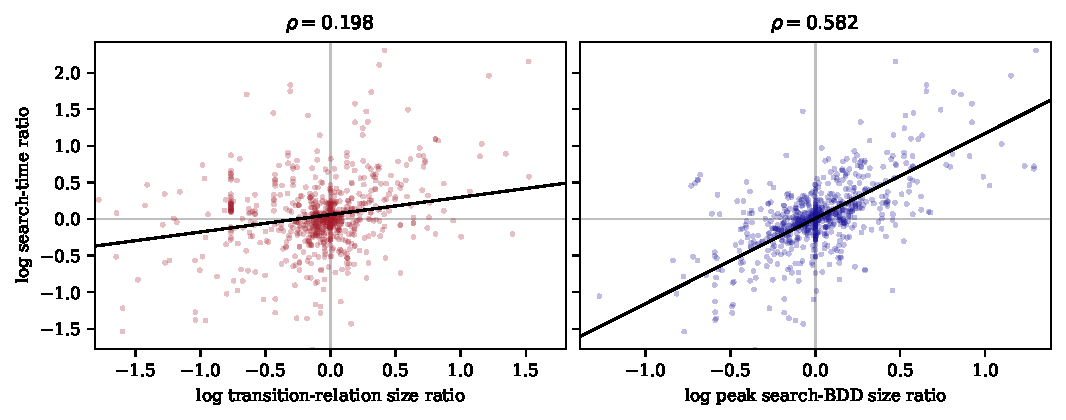
\includegraphics[width=0.86\textwidth]{mechanism.pdf}
\caption{\textbf{Why the ordering does not pay off: it moves the wrong quantity.}
Each point is one instance on which the method is active and both configurations
solve ($n = 759$); axes are log ratios of constraint-aware ordering to the
\textsf{GAMER} baseline, with the least-squares trend in black. \textbf{Left:}
the transition-relation size the objective actually optimizes barely predicts
runtime ($\rho = 0.198$) -- a diffuse cloud around a nearly flat trend.
\textbf{Right:} peak search-BDD size, which the ordering leaves essentially
unchanged, predicts runtime strongly ($\rho = 0.582$). Shrinking the transition
relation is not shrinking the search.}
\label{fig:mechanism}
\end{figure*}

\begin{insightbox}[Core Empirical Discovery: Shrinking TR $\neq$ Shrinking Search]
Optimizing variable ordering for mutex co-occurrence reliably shrinks Transition Relations (TRs) by 13.3\%. However, TR size correlates weakly with search runtime ($\rho = 0.202$). Search runtime is instead strictly governed by peak search-BDD node count ($\rho = 0.593$), which the ordering leaves uncompressed.
\end{insightbox}

\subsection{Empirical Ceiling Bounds \& Portfolio Selection Limits}
\label{sec:ceiling}
We investigated whether algorithm selection, restart schedules, or portfolio wrappers could extract suite-wide gains from constraint-aware variable orderings. We established several theoretical and empirical ceiling bounds:

\begin{itemize}\setlength{\itemsep}{2pt}
    \item Protocol Resolution Limit: Replicate analysis across 290 same-batch pairs reveals an intrinsic runtime variance of $\text{sd}(\log \text{runtime}) = 0.196$, with 29\% of identical-configuration runs differing by $>20\%$ and coverage drifting by up to 28 instances between full suite runs. This imposes a strict $\pm 17$-instance resolution ceiling for suite-wide coverage claims -- a bound we confirmed the hard way: an earlier 551-instance sample suggested a $+3$ suite-wide gain that did not replicate at full scale. Suite-wide coverage differences below this floor should not be trusted regardless of their apparent direction.
    \item Oracle Bound: An ideal 2-ordering oracle selector yields a theoretical coverage gain of +12 instances, which sits entirely below the $\pm 17$-instance noise floor. Calibrated models for $k$-ordering oracles yield +20 ($k=3$), +24 ($k=4$), +29 ($k=6$), and +33 ($k=8$) instances; practical selectors capturing $\sim \frac{1}{3}$ of oracle value cannot achieve statistically detectable suite-wide wins.
    \item Restart Schedules: In sequential budget-splitting tests under an 1800\,s limit, zero stock-unsolved instances are rescued by the constraint ordering within 600\,s, while 48 solved instances require $>900\,\text{s}$. Consequently, all tested budget splits reduce overall coverage.
    \item TR-Probe Selection: A build-time probe selector evaluating initial TR node size selects the correct ordering 70.8\% of the time \emph{when it deviates from stock} ($p = 5.4 \cdot 10^{-4}$, replicated at 71.2\%). Measured end-to-end, however, the probe tax dominates: the selector is \textbf{18.4\% slower} than stock in wall-clock (Table~\ref{tab:suitewide_results}), and no configuration in a 150-point parameter sweep is net-positive. Its nominal $+5$ coverage (1150 vs.\ 1145) lies well inside the $\pm 17$-instance noise floor and is not a claim we make.
\end{itemize}

\subsection{Methodological Findings}
Our investigation revealed two methodological insights for automated planning evaluations:

\subsubsection{Demonstration of Regression to the Mean}
Selecting "hard" instances based on baseline runtime artificially skews comparative speedup claims. Filtering instances where stock \textsf{SymK} takes $>10\,\text{s}$ makes constraint ordering appear 20\% faster (runtime ratio 0.796). Conversely, filtering by constraint ordering runtime makes it appear 6\% slower (ratio 1.064). A symmetric estimator yields a true ratio of 0.908 (54.5\% win rate). Standard asymmetric "hard instance" subsetting produces pure regression-to-the-mean artifacts.

\subsubsection{IPC Cross-Year Duplicate Leakage}
Evaluating static machine learning selectors via leave-one-domain-out cross-validation produced an apparent model fit of $R^2 = 0.30$. However, performance collapsed to $R^2 = -0.05$ under leave-one-\textit{family}-out cross-validation. Forensic analysis revealed that the IPC benchmark suite contains 299 cross-year duplicate instances (108 bit-identical tasks across 123 duplicate sets) that leak across domain splits, necessitating rigorous deduplication before learning.

\begin{table*}[t]
\centering

% ==================== TABLE 1 ====================
\caption{Pre-registered confirmatory A/B evaluation results (480 total runs across 2 independent replicates).}
\label{tab:prereg_ab}
\small
\begin{tabular}{llcc}
\toprule
\textbf{Pre-Registered Gate} & \textbf{Target Requirement} & \textbf{Empirical Outcome} & \textbf{Status} \\
\midrule
Primary: Coverage Contrast & Coverage Gain $\ge +4$ & \textbf{+6 (Rep 1) / +6 (Rep 2)} & \textbf{CONFIRMED} \\
Secondary: Woodworking Speed & Wall Time Geomean $\le 0.85$ & \textbf{0.647} ($1.55\times$ speedup, $n=94$) & \textbf{CONFIRMED} \\
Guard: Domain Losses & No Replicated Domain Loss & \textbf{0 Replicated Domain Losses} & \textbf{PASSED} \\
Integrity: Plan Optimality & 0 Cost Mismatches & \textbf{0 / 480 Cost Mismatches} & \textbf{PASSED} \\
\bottomrule
\end{tabular}

\vspace{2.5em}

% ==================== TABLE 2 ====================
\caption{Per-domain coverage breakdown on the five signal domains across Replicates 1 and 2. Counts are instances solved within 1800\,s; $|\mathcal{I}|$ is the number of instances in the domain.}
\label{tab:ab_domain_breakdown}
\small
\begin{tabular}{lccccc}
\toprule
\textbf{Domain} & \textbf{Weight $w_{\text{co}}$} & $\mathbf{|\mathcal{I}|}$ & \textbf{Stock (R1/R2)} & \textbf{Policy (R1/R2)} & \textbf{Coverage $\Delta$} \\
\midrule
\textit{parking-opt14-strips} & 1.0 & 20 & 1 / 0 & 3 / 3 & \textbf{+2 / +3} \\
\textit{barman-opt11-strips} & 1.0 & 20 & 9 / 9 & 10 / 11 & \textbf{+1 / +2} \\
\textit{tpp} & 1.0 & 30 & 8 / 8 & 9 / 9 & \textbf{+1 / +1} \\
\textit{woodworking-opt08-strips} & 2.0 & 30 & 27 / 28 & 28 / 28 & \textbf{+1 / +0} \\
\textit{woodworking-opt11-strips} & 2.0 & 20 & 19 / 20 & 20 / 20 & \textbf{+1 / +0} \\
\midrule
\textbf{Total Signal Domains} & -- & \textbf{120} & \textbf{64 / 65} & \textbf{70 / 71} & \textbf{+6 / +6} \\
\bottomrule
\end{tabular}

\vspace{2.5em}

% ==================== TABLE 3 ====================
\caption{Suite-wide performance across all 1,847 IPC optimal-STRIPS instances (repaired dataset). Time ratios are \textbf{wall-clock relative to stock}, including all selector probe overhead, over instances solved by both the row configuration and stock; intervals are domain-clustered bootstrap 95\% CIs. The selector's search-only ratio, which excludes its probe tax, is 0.992 -- its entire deficit is probe overhead.}
\label{tab:suitewide_results}
\small
\begin{tabular}{lccccc}
\toprule
\textbf{Configuration} & \textbf{Coverage} & \textbf{Geomean Wall Ratio} & \textbf{Median Ratio} & \textbf{95\% Conf. Interval} & $\mathbf{n}$ \\
\midrule
Stock \textsf{SymK} (Baseline) & 1145 & 1.0000 & 1.0000 & -- & -- \\
Always-On Constraint Ordering & 1139 & 1.0053 & 1.0000 & [0.97, 1.05] & 1126 \\
TR-Probe Selector & 1150 & 1.1837 & 1.1740 & [1.16, 1.21] & 1141 \\
\bottomrule
\end{tabular}
\end{table*}

\section{Discussion \& Related Work}
Our findings touch upon several foundational threads in symbolic classical planning, constraint-graph variable ordering, algorithm selection, and empirical research methodology.

\subsection{Symbolic Search and BDD Variable Ordering}
Symbolic state-space exploration relies on Binary Decision Diagrams (BDDs) to represent state sets and transition relations compactly. The computational cost of symbolic search is dictated by the BDD node count, which is notoriously sensitive to the chosen variable ordering. \textsf{GAMER} \cite{edelkamp2008gamer} introduced local search over a weighted linear arrangement objective on causal graph edges to optimize BDD variable orders. This scheme was inherited largely unchanged by state-of-the-art planners, including \textsf{SymBA*} \cite{torralba2014symba} and \textsf{SymK} \cite{speck2020symk, speck2023symkipc}.

Kissmann and Hoffmann \cite{kissmann2014bdd} conducted an extensive study of BDD variable orderings in classical planning, establishing that ordering quality can vary wildly across instances and that finding optimal orderings statically is highly unpredictable. Our diagnostic results reinforce their verdict of unpredictability: while constraint-aware ordering systematically compresses transition relations (TRs), search runtime is ultimately governed by the peak search-BDD size, which is unaffected by preprocessing-time topology optimizations.

\subsection{Invariants and Constraint-Aware Ordering}
The inclusion of state invariants, such as $h^2$ mutexes and exactly-one groups, is essential for pruning spurious states during symbolic search frontier expansion \cite{torralba2013constrained}. Torralba and Alc\'azar \cite{torralba2013constrained} observed that these conjoined constraint BDDs depend heavily on the variable ordering and explicitly suggested incorporating mutex edges into the arrangement objective as future work. Our work directly implements and evaluates this open suggestion inside \textsf{SymK}.

Outside classical planning, constraint-graph variable ordering is well-established in SAT and VLSI CAD literature, exemplified by force-directed heuristics like \textsf{FORCE} and \textsf{MINCE} \cite{aloul2003force}. While approaches like \textsf{GamerPre} \cite{kissmann2014bdd} incorporate precondition co-occurrence edges, and Torralba et al.\ \cite{torralba2017efficient} use mutexes and invariants for pruning and constraint-BDD compilation while holding the variable order fixed, our framework specifically targets state-invariant mutex and invariant group co-occurrences within the \textsf{GAMER} arrangement objective itself.

\subsection{Algorithm Selection, Portfolios, and Methodology}
Per-instance algorithm selection and sequential portfolios (e.g., \textsf{SATzilla} \cite{xu2008satzilla}, Fast Downward Stone Soup \cite{helmert2011stonesoup}) are standard techniques for navigating solver complementary strengths. Our ceiling bound analysis demonstrates why standard selection or restart wrappers over these orderings fail to yield suite-wide gains: the theoretical two-ordering oracle gain (+12 instances) sits below our measured empirical protocol noise floor ($\pm 17$ instances).

Furthermore, our methodological findings contribute important cautionary lessons for planning benchmarks:
\begin{enumerate}\setlength{\itemsep}{1pt}
    \item \textbf{Regression to the Mean:} We demonstrated that evaluating runtime speedups strictly on "hard" instances filtered by baseline performance introduces severe selection bias, turning neutral performance into an apparent 20\% speedup.
    \item \textbf{Cross-Year Duplicate Leakage:} We identified 299 cross-year duplicate instances in the IPC benchmark suite, proving that domain-wise cross-validation leaks information across splits and inflates learned selector metrics ($R^2 = 0.30 \to -0.05$ under deduplication).
\end{enumerate}
Variable ordering was not our first target: we first explored search-control alternatives, including landmark-guided direction selection for bidirectional symbolic search, meet-in-the-middle BDD-overlap signals, and forward-reachability pruning of the backward frontier, all of which we found to be net-neutral or actively harmful, ultimately pointing us toward the variable-ordering lever explored in this paper.

\section{Conclusion \& Future Work}
In this paper, we implemented and evaluated constraint-aware variable ordering inside \textsf{SymK} across the complete IPC optimal-STRIPS benchmark suite. Our inquiry delivers four primary outcomes:

\begin{itemize}\setlength{\itemsep}{2pt}
    \item \textbf{Confirmed Per-Domain Advance:} A pre-registered, double-replicated A/B policy strictly improves stock \textsf{SymK} by \textbf{$+6$ coverage} (exactly replicated) across its five target domains and accelerates \textit{woodworking} by \textbf{$1.55\times$}, with zero plan cost mismatches.

    \item \textbf{Bounded Suite-Wide Null:} Enabled universally, the ordering yields a tightly bounded zero effect (coverage 1145 vs.\ 1139; geomean wall ratio 1.005, 95\% CI [0.97, 1.05]), excluding even a 5\% suite-wide effect.

    \item \textbf{Mechanism Uncovering:} Diagnostic logging reveals the root cause: the ordering systematically compresses Transition Relation (TR) node sizes by 13.3\% ($p \approx 3 \cdot 10^{-21}$), but TR size is decoupled from search cost ($\rho = 0.202, R^2 \approx 0.04$), which is instead dictated by peak search-BDD size ($\rho = 0.593$).

    \item \textbf{Ceiling Bounds \& Methodological Insights:} Empirical protocols establish a $\pm 17$-instance resolution limit, proving why portfolios and selection wrappers cannot yield suite-wide gains, while highlighting critical traps in hard-instance subsetting and IPC duplicate leakage.
\end{itemize}

\subsection{Future Directions}
Our diagnostic decoupling points directly toward two promising avenues for future research in symbolic search:

\subsubsection{Targeting Peak Search-BDD Size}
Because peak search-BDD node count is highly predictive of runtime ($\rho = 0.593$) and bit-deterministic across runs ($r = 0.999$), future variable ordering objectives should target peak search-BDD expansion directly. Since peak BDD sizes are unobservable during preprocessing, developing lightweight online probes or dynamic reordering criteria that estimate search-space width remains an open challenge.

\subsubsection{Exploiting Ordering Diversity}
Published random-ordering distributions exhibit heavy favorable tails that correlated structural orderings cannot reach \cite{kissmann2014bdd}. Designing randomized, high-diversity ordering portfolios paired with early-termination rerun controls could unlock the heavy-tail performance gains of symbolic BDD search.

\small
\bibliographystyle{plain}
\bibliography{references}

\end{document}
